
\paragraph{Per-Game Observations (Human‐Normalized)}
To illustrate performance trends for \textbf{PPO}, \textbf{REINFORCE}, and \textbf{SAC} in greater detail, Figures~\ref{fig:policy_comp_alien}--\ref{fig:policy_comp_pong} compare the three algorithms’ human‐normalized returns over \num{100000} steps for each of the eight Atari games under consideration.

% ---------------------------------------------------------
% ALIEN
\begin{figure}[htbp]
	\centering
	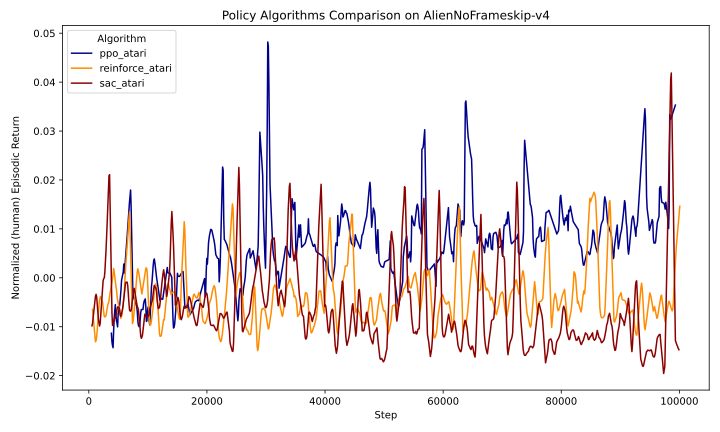
\includegraphics[width=0.45\textwidth]{figures/policy_comparison/charts_episodic_return_human_comparison_AlienNoFrameskip-v4_policy.png}
	\caption{\textbf{Alien (Human-Norm).} SAC (red) and PPO (blue) frequently hover near 0.0--0.02, with occasional spikes reaching 0.04--0.05. REINFORCE (orange) remains mostly near or below 0.0.}
	\label{fig:policy_comp_alien}
\end{figure}

\noindent
\textbf{Alien.} In Figure~\ref{fig:policy_comp_alien}, \textbf{PPO} (blue) and \textbf{SAC} (red) occasionally spike up to around 0.04--0.05, surpassing \textbf{REINFORCE} (orange), which lingers near zero or slightly negative. SAC sees a final jump near 100k steps, while PPO’s peaks are somewhat spread out across training.

% ---------------------------------------------------------
% AMIDAR
\begin{figure}[htbp]
	\centering
	\includegraphics[width=0.45\textwidth]{figures/policy_comparison/charts_episodic_return_human_comparison_AmidarNoFrameskip-v4_policy.png}
	\caption{\textbf{Amidar (Human-Norm).} PPO (blue) rises above 0.03 by 40k steps, reaching nearly 0.05. SAC (red) and REINFORCE (orange) remain mostly under 0.01.}
	\label{fig:policy_comp_amidar}
\end{figure}

\noindent
\textbf{Amidar.} Figure~\ref{fig:policy_comp_amidar} shows \textbf{PPO} far ahead, climbing past 0.03 around mid-training and peaking near 0.05 by 100k. In contrast, both \textbf{SAC} and \textbf{REINFORCE} rarely exceed 0.01, indicating limited improvement over random play within 100k steps.

% ---------------------------------------------------------
% ASSAULT
\begin{figure}[htbp]
	\centering
	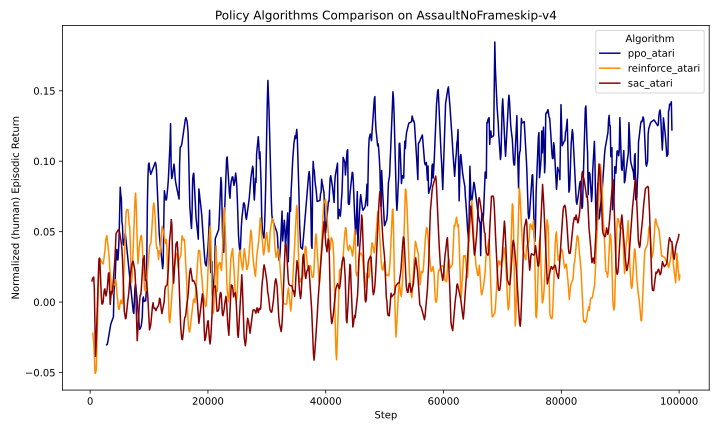
\includegraphics[width=0.45\textwidth]{figures/policy_comparison/charts_episodic_return_human_comparison_AssaultNoFrameskip-v4_policy.png}
	\caption{\textbf{Assault (Human-Norm).} PPO (blue) reaches 0.15--0.18 near the end, SAC (red) hovers around 0.05--0.10, and REINFORCE (orange) stays below 0.05.}
	\label{fig:policy_comp_assault}
\end{figure}

\noindent
\textbf{Assault.} Figure~\ref{fig:policy_comp_assault} confirms \textbf{PPO}’s dominance again, steadily rising above 0.15 by 100k steps. \textbf{SAC} manages intermediate returns (0.05--0.10), while \textbf{REINFORCE} remains under 0.05. SAC’s line is more stable here than in some other games, but never surpasses PPO’s peak.

% ---------------------------------------------------------
% BOXING
\begin{figure}[htbp]
	\centering
	\includegraphics[width=0.45\textwidth]{figures/policy_comparison/charts_episodic_return_human_comparison_BoxingNoFrameskip-v4_policy.png}
	\caption{\textbf{Boxing (Human-Norm).} REINFORCE (orange) hits extreme spikes above +2, but also dips below -1.5. SAC (red) fluctuates similarly, and PPO (blue) ranges from about -1.0 to +1.0.}
	\label{fig:policy_comp_boxing}
\end{figure}

\noindent
\textbf{Boxing.} In Figure~\ref{fig:policy_comp_boxing}, \emph{all three} algorithms show \emph{extreme variance}. \textbf{REINFORCE} (orange) occasionally spikes above 2.0, offset by negative dips below -1.5. \textbf{SAC} (red) also oscillates widely, while \textbf{PPO} (blue) spans roughly -1.0 to +1.0. This environment heavily influences SAC’s negative overall mean (see Table~\ref{tab:policy_final_eval_human}).

% ---------------------------------------------------------
% BREAKOUT
\begin{figure}[htbp]
	\centering
	\includegraphics[width=0.45\textwidth]{figures/policy_comparison/charts_episodic_return_human_comparison_BreakoutNoFrameskip-v4_policy.png}
	\caption{\textbf{Breakout (Human-Norm).} SAC (red) scales up to 0.4--0.55 near 100k steps. PPO (blue) and REINFORCE (orange) rarely exceed 0.1--0.15.}
	\label{fig:policy_comp_breakout}
\end{figure}

\noindent
\textbf{Breakout.} Figure~\ref{fig:policy_comp_breakout} demonstrates a strong showing by \textbf{SAC}, which begins modestly but eventually outperforms both \textbf{PPO} and \textbf{REINFORCE}. By around 60k steps, SAC’s returns surpass 0.2--0.3, and near 100k steps it reaches 0.5 or higher. PPO (blue) oscillates around 0.1--0.2, and REINFORCE (orange) stays mostly under 0.1.

% ---------------------------------------------------------
% FREEWAY
\begin{figure}[htbp]
	\centering
	\includegraphics[width=0.45\textwidth]{figures/policy_comparison/charts_episodic_return_human_comparison_FreewayNoFrameskip-v4_policy.png}
	\caption{\textbf{Freeway (Human-Norm).} PPO (blue) climbs steadily past 0.15--0.18, while both REINFORCE (orange) and SAC (red) remain near 0.0.}
	\label{fig:policy_comp_freeway}
\end{figure}

\noindent
\textbf{Freeway.} As shown in Figure~\ref{fig:policy_comp_freeway}, \textbf{PPO} significantly outperforms the other two methods, rising to about 0.18--0.20 by 100k steps. \textbf{REINFORCE} (orange) makes a brief jump near 0.01--0.02 around 15k steps, but then stagnates. \textbf{SAC} (red) essentially hovers around 0.0 throughout.

% ---------------------------------------------------------
% MS PAC-MAN
\begin{figure}[htbp]
	\centering
	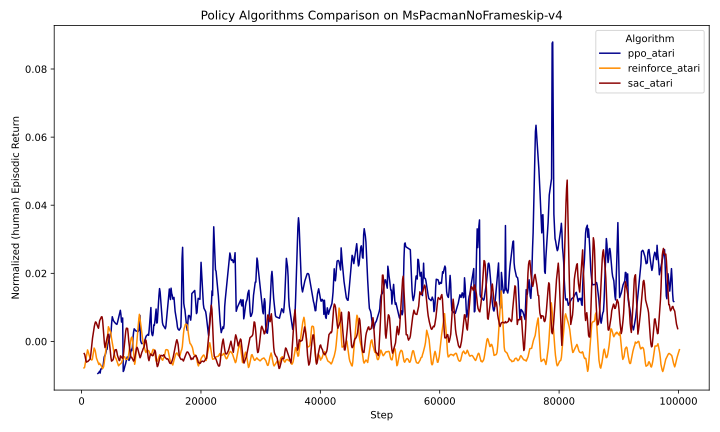
\includegraphics[width=0.45\textwidth]{figures/policy_comparison/charts_episodic_return_human_comparison_MsPacmanNoFrameskip-v4_policy.png}
	\caption{\textbf{MsPacman (Human-Norm).} PPO (blue) eventually spikes near 0.08. SAC (red) remains at 0.03--0.05, and REINFORCE (orange) stays below 0.02.}
	\label{fig:policy_comp_mspacman}
\end{figure}

\noindent
\textbf{MsPacman.} In Figure~\ref{fig:policy_comp_mspacman}, \textbf{PPO} again leads, peaking around 0.08 near 80k steps. \textbf{SAC} tracks behind, mostly in the 0.02--0.05 range. \textbf{REINFORCE} remains under 0.02, showing minimal gains after 100k interactions.

% ---------------------------------------------------------
% PONG
\begin{figure}[htbp]
	\centering
	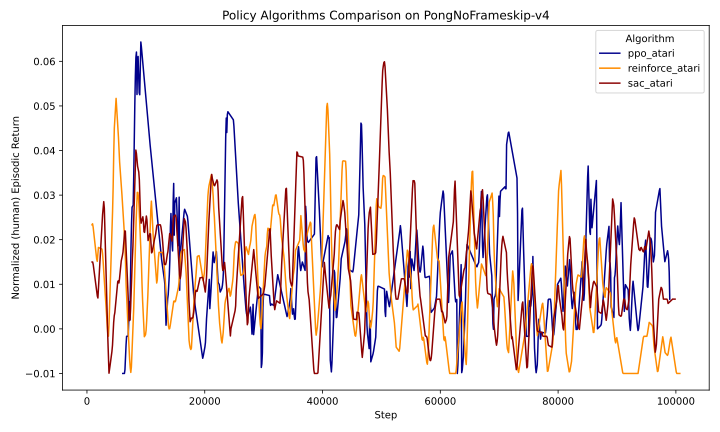
\includegraphics[width=0.45\textwidth]{figures/policy_comparison/charts_episodic_return_human_comparison_PongNoFrameskip-v4_policy.png}
	\caption{\textbf{Pong (Human-Norm).} All three fluctuate around 0.0--0.06. PPO (blue) occasionally spikes to 0.06, while REINFORCE (orange) and SAC (red) show comparable swings.}
	\label{fig:policy_comp_pong}
\end{figure}

\noindent
\textbf{Pong.} Finally, Figure~\ref{fig:policy_comp_pong} indicates \emph{no strong lead} for any single algorithm. \textbf{PPO} and \textbf{REINFORCE} see sporadic spikes around 0.04--0.06, but remain near 0.0 most of the time. \textbf{SAC} likewise oscillates in a similar band. Overall, none of the policy gradient approaches achieve notable improvement within just 100k steps in this game.

\smallskip
\noindent
\textbf{Takeaways Across All Games.}  
- \textbf{PPO} often attains the highest or second-highest returns in most environments except \emph{Breakout}, where \textbf{SAC} excels.  
- \textbf{SAC} exhibits strong late-game gains in \emph{Breakout} and moderate performance in \emph{Assault}, but struggles in \emph{Freeway} and is highly volatile in \emph{Boxing}.  
- \textbf{REINFORCE} remains comparatively weak in most tasks, with occasional spikes in \emph{Boxing} but minimal improvements elsewhere, underscoring the challenges of pure Monte Carlo policy gradients within only 100k steps.

\paragraph{Per-Game Observations (Min--Max Normalized)}

In addition to the human‐normalized curves, we compare these three policy gradient algorithms under \textbf{min--max normalization}, which rescales each environment’s returns based on its observed minimum and maximum. This viewpoint can clarify differences that might be overshadowed by large raw score ranges.

\medskip

\textbf{Alien.}
\begin{figure}[htbp]
	\centering
	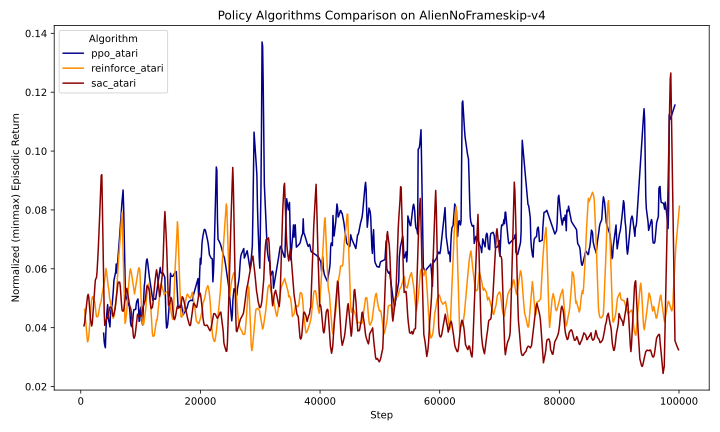
\includegraphics[width=0.45\textwidth]{figures/policy_comparison/charts_episodic_return_minmax_comparison_AlienNoFrameskip-v4_policy.png}
	\caption{\textbf{Alien (Min--Max).} PPO (blue) periodically spikes near 0.12--0.14, while SAC (red) follows closely toward 100k. REINFORCE (orange) mostly remains around 0.04--0.08.}
	\label{fig:policy_minmax_alien}
\end{figure}

Figure~\ref{fig:policy_minmax_alien} shows \textbf{PPO} reaching the highest peaks, above 0.12 around 50--60k steps and near 100k, whereas \textbf{SAC} (red) tends to track just below but manages a final jump late in training. \textbf{REINFORCE} (orange) stays lower overall, in the 0.04--0.08 band.

\medskip

\textbf{Amidar.}
\begin{figure}[htbp]
	\centering
	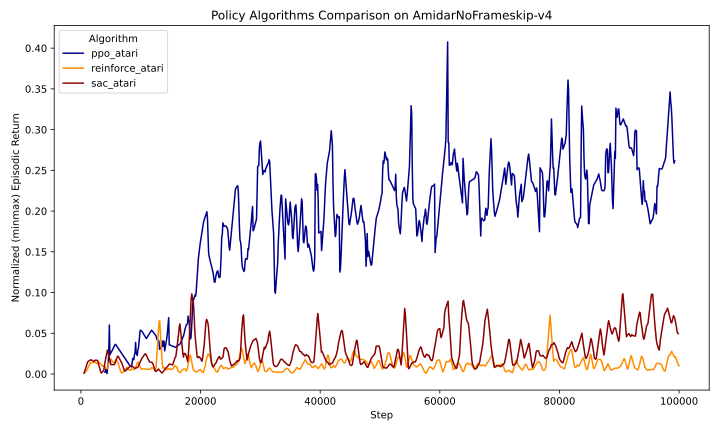
\includegraphics[width=0.45\textwidth]{figures/policy_comparison/charts_episodic_return_minmax_comparison_AmidarNoFrameskip-v4_policy.png}
	\caption{\textbf{Amidar (Min--Max).} PPO (blue) quickly exceeds 0.20, reaching over 0.35 near 80k. SAC (red) and REINFORCE (orange) remain mostly below 0.1.}
	\label{fig:policy_minmax_amidar}
\end{figure}

In Figure~\ref{fig:policy_minmax_amidar}, \textbf{PPO} again stands out, crossing 0.30 around mid‐training and eventually nearing 0.35. \textbf{SAC} (red) and \textbf{REINFORCE} (orange) struggle to exceed 0.1, indicating minimal progress relative to Amidar’s observed max returns.

\medskip

\textbf{Assault.}
\begin{figure}[htbp]
	\centering
	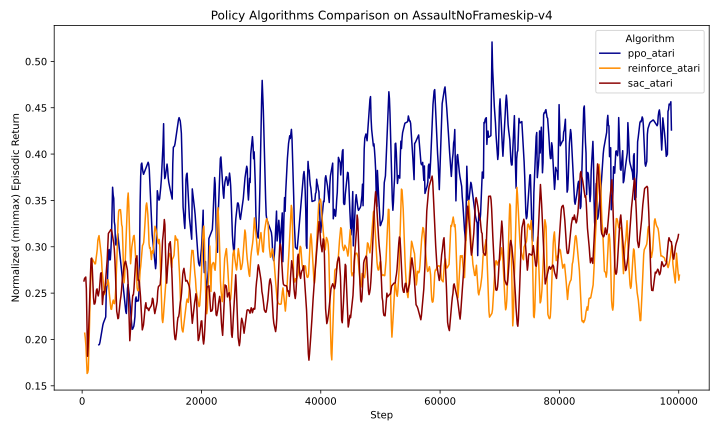
\includegraphics[width=0.45\textwidth]{figures/policy_comparison/charts_episodic_return_minmax_comparison_AssaultNoFrameskip-v4_policy.png}
	\caption{\textbf{Assault (Min--Max).} PPO (blue) hovers between 0.30--0.50, while SAC (red) and REINFORCE (orange) cluster around 0.20--0.35.}
	\label{fig:policy_minmax_assault}
\end{figure}

From Figure~\ref{fig:policy_minmax_assault}, \textbf{PPO} maintains a clear advantage (0.30--0.50), whereas \textbf{SAC} (red) and \textbf{REINFORCE} (orange) seldom surpass 0.35. This is consistent with the pattern seen under human normalization.

\medskip

\textbf{Boxing.}
\begin{figure}[htbp]
	\centering
	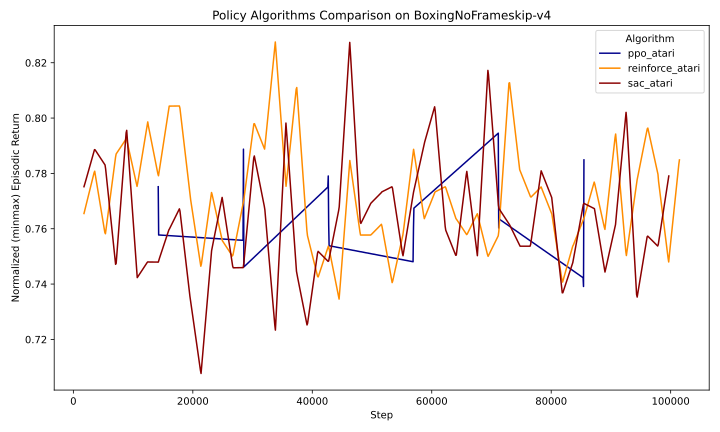
\includegraphics[width=0.45\textwidth]{figures/policy_comparison/charts_episodic_return_minmax_comparison_BoxingNoFrameskip-v4_policy.png}
	\caption{\textbf{Boxing (Min--Max).} All three algorithms reside in a narrow 0.72--0.82 range, reflecting that large raw score swings translate to a relatively small fraction of the total possible range.}
	\label{fig:policy_minmax_boxing}
\end{figure}

Figure~\ref{fig:policy_minmax_boxing} shows that, unlike the wide swings in human‐normalized space, all methods remain clustered around 0.72--0.82. \textbf{REINFORCE} (orange) sometimes peaks near 0.83, \textbf{SAC} (red) around 0.80, and \textbf{PPO} (blue) near 0.75--0.80.

\medskip

\textbf{Breakout.}
\begin{figure}[htbp]
	\centering
	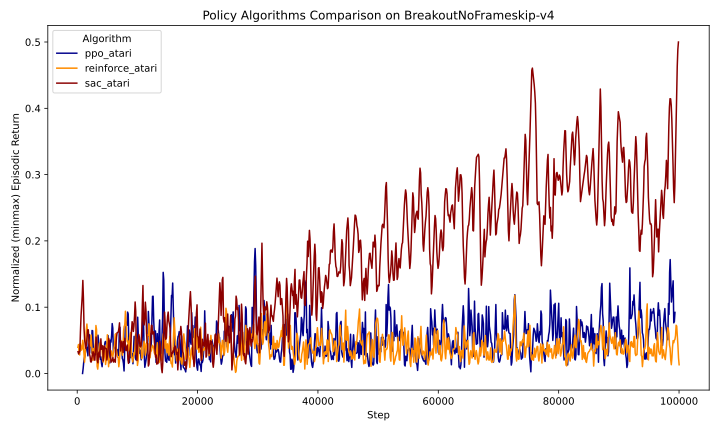
\includegraphics[width=0.45\textwidth]{figures/policy_comparison/charts_episodic_return_minmax_comparison_BreakoutNoFrameskip-v4_policy.png}
	\caption{\textbf{Breakout (Min--Max).} SAC (red) climbs from ~0.1 to over 0.4 by 80k steps, ultimately exceeding 0.5 at 100k. PPO (blue) hovers around 0.2, REINFORCE (orange) below 0.1.}
	\label{fig:policy_minmax_breakout}
\end{figure}

As in the human‐norm perspective, \textbf{SAC} surges significantly in Breakout, starting modestly but surpassing 0.3--0.4 around 60--70k steps, ultimately topping 0.5 near the end. \textbf{PPO} floats around 0.1--0.2, and \textbf{REINFORCE} remains under 0.1.

\medskip

\textbf{Freeway.}
\begin{figure}[htbp]
	\centering
	\includegraphics[width=0.45\textwidth]{figures/policy_comparison/charts_episodic_return_minmax_comparison_FreewayNoFrameskip-v4_policy.png}
	\caption{\textbf{Freeway (Min--Max).} PPO (blue) nearly monotonically ascends to 0.20 by 100k, while SAC (red) and REINFORCE (orange) remain near 0.0.}
	\label{fig:policy_minmax_freeway}
\end{figure}

In Figure~\ref{fig:policy_minmax_freeway}, \textbf{PPO} soars to around 0.20, yet \textbf{SAC} (red) and \textbf{REINFORCE} (orange) barely budge from 0.0--0.01, highlighting the high maximum potential of Freeway relative to their minimal score gains.

\medskip

\textbf{MsPacman.}
\begin{figure}[htbp]
	\centering
	\includegraphics[width=0.45\textwidth]{figures/policy_comparison/charts_episodic_return_minmax_comparison_MsPacmanNoFrameskip-v4_policy.png}
	\caption{\textbf{MsPacman (Min--Max).} PPO (blue) spikes near 0.35--0.40 around 80k, with SAC (red) at 0.15--0.20, and REINFORCE (orange) below 0.10.}
	\label{fig:policy_minmax_mspacman}
\end{figure}

Figure~\ref{fig:policy_minmax_mspacman} shows \textbf{PPO} again in the lead, reaching 0.35--0.40. \textbf{SAC} (red) hovers around 0.20, while \textbf{REINFORCE} (orange) rarely exceeds 0.10. These proportions match the human‐norm results, but with clearer numeric gaps.

\medskip

\textbf{Pong.}
\begin{figure}[htbp]
	\centering
	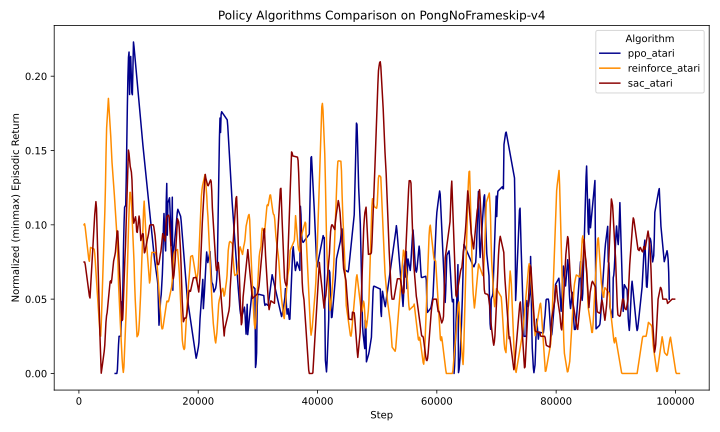
\includegraphics[width=0.45\textwidth]{figures/policy_comparison/charts_episodic_return_minmax_comparison_PongNoFrameskip-v4_policy.png}
	\caption{\textbf{Pong (Min--Max).} None of the algorithms achieve substantial gains, oscillating around 0.0--0.2.}
	\label{fig:policy_minmax_pong}
\end{figure}

Finally, Figure~\ref{fig:policy_minmax_pong} reveals that \textbf{PPO}, \textbf{SAC}, and \textbf{REINFORCE} all produce limited improvements, fluctuating between 0.0 and 0.2 throughout the 100k steps.

\medskip
\noindent
\textbf{Overall Min--Max Observations.}  
Taken together, these \textbf{min--max} curves mirror many of the same takeaways from the \emph{human‐normalized} plots:
\begin{itemize}
	\item \textbf{PPO} dominates or competes favorably in most environments, especially \emph{Amidar}, \emph{Assault}, \emph{Freeway}, and \emph{MsPacman}. 
	\item \textbf{SAC} excels in \emph{Breakout} and remains reasonably strong in \emph{Alien} or \emph{Assault}, though it stalls in \emph{Freeway} and \emph{Pong}.
	\item \textbf{REINFORCE} typically underperforms, staying below 0.1--0.2 in most games with the rare exception of \emph{Boxing} (though that game’s min–max scale is narrow).
\end{itemize}
Hence, PPO generally emerges as the most consistently successful policy gradient approach in this short 100k‐interaction benchmark, with SAC showing pockets of promise but higher variance, and REINFORCE lagging significantly in most tasks.